\subsection{T3 Task 3. Code Coverage RL, Relation RL, and CRL for Fault Localization}

\begin{wrapfigure}{r}{0.45\textwidth}
	\vspace{-12pt}
	\centering
	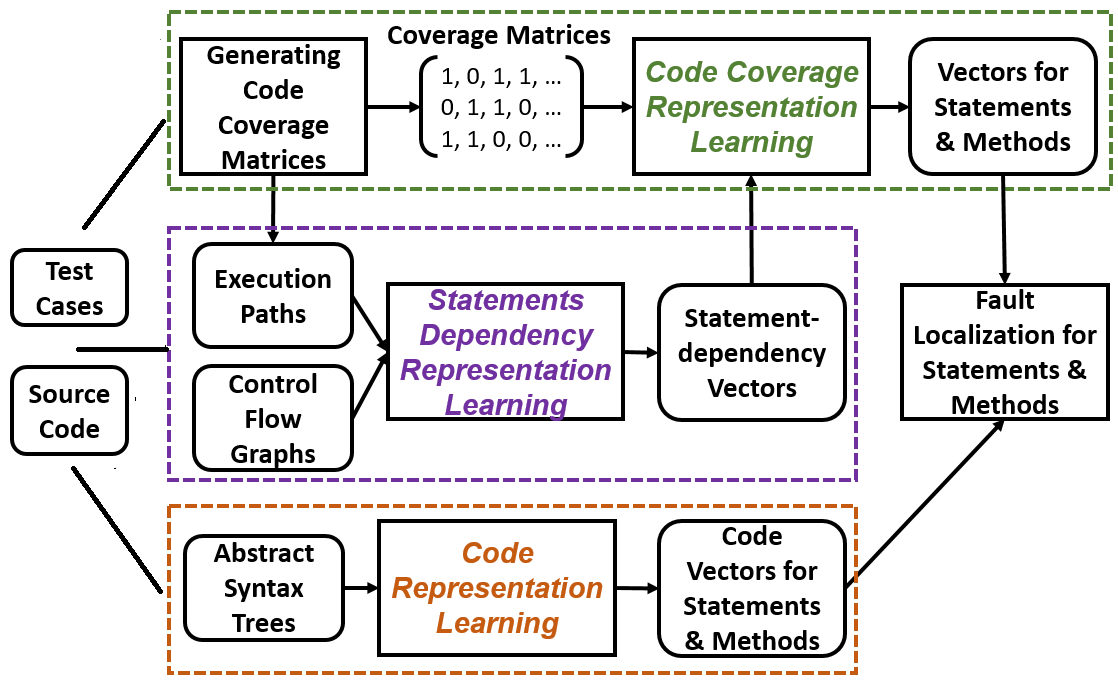
\includegraphics[height=1.8in]{graphs/newOverview}
	\vspace{-20pt}
	\caption{Using Representation Learning in FL.}
	\label{floverview}
	\vspace{-10pt}
\end{wrapfigure}
To experiment with CRL for dynamic information from program
executions, we propose a customized CRL for a fault localization
approach~\cite{icse_fl_21} at the statement and method levels.
%
%We use effective code and test coverage representation learning and
%novel deep neural networks for localizing faults at statement and
%method levels.
Our preliminary design~\cite{icse_fl_21} (Figure~\ref{floverview}) was
to leverage representation learning (RL) in three aspects. (1) {\bf
  code coverage representation learning}: Existing approaches
(spectrum-based, mutation-based, and deep learning-based approaches)
have never used the full details of test coverage, instead, they use
the spectrum and(or) mutation based formulas to summarize test
coverage for all test cases on each statement. We propose to {\em
  treat the FL problem as image processing by learning code coverage
  representations on the full details of the test coverage matrix}.
%Existing approaches (spectrum-based, mutation-based, and deep
%learning-based approaches) have never used the full details of test
%coverage, instead, they use the spectrum and(or) mutation based
%formulas to summarize test coverage for all test cases on each
%statement.
%To enrich test coverage matrices, we extract failing information of a
%test case and link it with specific code statements.  We use -1 for a
%failing test case at a statement exhibiting a crash or incorrect
%value.
%
%Next, while the rows representing statements are arranged according to
%the appearance order in the code, we order the columns, representing
%the test cases, so that the test coverages (i.e., the -1s, 0s, and 1s
%in the test coverage matrix) around the buggy statement would form a
%characteristic ``visual'' feature for a DL model to learn and detect
%it.  We directly perform RL on the improved matrices to learn vectors
%for statements or methods.  \underline{Second}, we integrate the
%dependencies/relations among the statements in the fault localization
%process using data dependency and execution traces.
(2) {\bf Statement dependency representation learning}: we aim to
learn the data/control dependencies among the statements. (3) {\bf
  code representation learning}: we also conduct CRL on sub-trees and
long paths of ASTs to generate vectors for source code. Finally, we
combine all three types of representation learning to represent a
statement or method by a vector representation. We will explore
different DL models for the classification purpose.~Preliminary
work shows that CNN works well for this classification of
a method/statement into buggy or not.

%(1) We prioritize test cases and mine failing information of test
%cases to enrich test coverage matrices and learn the code coverage
%representations; (2) We conduct the CRL on sub-trees and long paths of
%ASTs to generate vectors for source code, and also generate data flow
%graphs and run test cases to collect execution paths of code
%statements to learn the statement dependencies; (3) We combine the
%data flow graph and execution paths with improved matrices (spectrum
%and mutation), then apply a \cnn~on new matrices to learn vectors for
%an improved matrix.  We use another CNN on code vectors, vectors for
%the improved spectrum--based matrices, and vectors for the improved
%mutation-based matrices to perform fault localization (FL) at
%method-level. Our design can also work on statement-level FL by
%replacing the CRL at statement-level.


%\begin{table}[h]
%	\vspace{-15pt}
%	
%	{\footnotesize	
%		\caption{Our Approach Compared with FL Baselines at method-level and statement-level on Defects4J having 395 Bugs in total}
%		\begin{center}
%			\renewcommand{\arraystretch}{1}
%			\begin{tabular}{p{1cm}<{\centering}|p{0.8cm}<{\centering}|p{1cm}<{\centering}p{1cm}<{\centering}p{1cm}<{\centering}p{1.5cm}<{\centering}
%					p{1.2cm}<{\centering}p{1.5cm}<{\centering}|p{1.6cm}<{\centering}p{1.5cm}<{\centering}p{0.8cm}<{\centering}p{1.2cm}<{\centering}|p{0.8cm}<{\centering}} \cline{2-13}				\hline
%				\multirow{2}{*}{}& \multicolumn{7}{c|}{Fault Localization at Statement-Level} & \multicolumn{5}{c}{Fault Localization Method-Level}\\
%				\cline{2-13}
%				& \textbf{Ours} & \textbf{Ochiai} & \textbf{Dstar} & \textbf{MUSE} & \textbf{Metallaxis} &\textbf{RBF-NN} & \textbf{DeepFL-S} &\textbf{MULTRIC} & \textbf{FLUCCS} & \textbf{TraPT} & \textbf{DeepFL}&\textbf{Ours}\\
%				\hline
%				Top-1  & \textbf{74} & 17 & 19 & 26 & 24   & 16 & 36 & 80 & 160  & 156 & 213 &    \textbf{242} \\
%				MFR & \textbf{19.97}& 46.51 & 39.47 & 32.51 & 31.42 & 20.96 & 21.89  & 37.71 & 16.53 & 9.94 & 6.63 & \textbf{6.21}\\
%				\hline
%			\end{tabular}
%			RBF-NN: RBF Neural Network,
%			DeepFL-S: DeepFL with only features from spectrum+Mutation+MLP applicable to statements,
%			Top-1: the number of faults with a least one faulty element (statement or method) within top-1 position,
%			MFR: Mean First Rank of the localization of the first faulty element.
%			All method-level FL are machine learning (incl. deep learning) based.
%			\label{FL_S_M}
%		\end{center}
%		\vspace{-20pt}
%	}
%\end{table}


%Table~\ref{FL_S_M} show that our initial approach outperformed all baselines at both statement and method levels. Compared with the best performing statement-level and method-level baseline: DeepFL-S and DeepFL, we improved them by 115\% and 14\%, respectively. Our key ideas of designing representation learning for code and test coverage can help improve the current state-of-the-art FL research.

%To expand our initial design, we will (1) derive new code representations for FL; (2) Explore new embeddings and learning models to propose new code representation learning (CRL) approaches for FL; (3) Study and proposing new deep neural networks to localize faults.

\subsection{T3 Task 4. Code Transformation Learning for Automated Program Repair}

In this task, we aim to improve DL-based APR approaches via effective
CRLs, particularly {\bf Code Transformation Learning}.
%to improve the current deep-learning (DL) and pattern APR approaches
%using effective CRL and novel deep neural networks.  The DL-based
%approaches, e.g.,~\cite{hata2018learning,lutellier2020coconut}, still
%have limitations in learning bug-fixing code changes and learning
%which context of the surrounding source code that certain bug-fixing
%changes should be made.  These limitations lead to incorrect fixing
%locations or incorrect fixes.
We initially designed a two-tier DL model, \tool~\cite{icse_fl_20}, to
treat APR as code transformation learning from the prior bug fixes and
the surrounding code contexts of the fixes.
%
%For training, {\tool} has 5 key steps: {\bf (1) Pre-Processing.}
%First, {\tool} performs alpha-renaming on the names of variables
%within a method of a project.  Second, , {\tool} uses
%Word2Vec~\cite{Mikolov-2013} to train a vector representation for each
%unique token in a given pair of buggy method ($M_b$) and its fixed
%version ($M_f$).  {\tool} identifies the buggy sub-tree ($T^{sub}_b$)
%within $M_b$, and $T^{sub}_b$'s corresponding changed sub-tree
%($T^{sub}_f$) within $M_f$.  Finally, we used a code summarization
%model~\cite{wan-ase18} to summarize a tree into a vector for a node
%({\em a summarized node}). We obtain one vector for $T^{sub}_f$ and
%another one for $T^{sub}_b$.
{\bf (1) Code Context Learning.} We designed a two-layer learning model
that leans the code transformations for bug fixes and the context of
the code surrounding the fixes. The first one is dedicated for local
\textbf{C}ontext \textbf{L}earning \textbf{L}ayer (CLL).
%
For training at this layer, we replace the changed sub-tree with
a {\em summarized node}, as well as the buggy
sub-tree.  Given pre-processed pairs of methods, we developed a
tree-based encoder-decoder model using tree-based
LSTMs~\cite{tai2015improved} for this local context learning.  We
compute the vector for a method AST with the summarized node in a pair
of methods ($M_b$, $M_f$). The obtained vectors are used as the weights
in the next step. {\bf (2) Code Transformation
	Learning.}  The second layer is dedicated to code
\textbf{T}ransformation \textbf{L}earning \textbf{L}ayer (TLL) for
bug-fixing changes. In TTL, the changed sub-tree before and after the
fix is used for training to learn the bug-fixing code
transformations. Moreover, the context of the transformation computed
as the vector in the context learning layer is used as an additional
input in this~step.
%Specifically, we use the same tree-based encoder-decoder model in the
%first layer, CLL, to encode both structural and token changes.  {\bf
%  (4) Program Analysis Filtering.}  {\tool} derives the possible
%candidates using program analysis filters, including the filter to
%check the existence of variables, methods, and class names, the filter
%to convert the keywords back to the right names, and the filter to
%check the syntax of final result.  {\bf (5) Patch Re-ranking.} We use
%a CNN~\cite{kim2014convolutional} based classification approach to
%re-rank the generated possible patches based on the detailed
%contextual information, which helps better selecting the results.

We also have the following tasks in this thrust: (1) Investigating new
code representations for APR using our code representation learning
(CRL) framework; (2) Exploring new embeddings and learning
models to propose new CRL approaches specialized for APR; and (3)
Studying and even proposing new deep neural network models to auto-fix
multi-statements and multi-location bugs.

%In our initial design, our DLFix is novel in two ways: new CRL and a
%new two-layer tree-based encoder-decoder model.
